\documentclass[12pt]{article} 
\usepackage[utf8]{inputenc}
\usepackage{geometry}
\geometry{letterpaper}
\usepackage{graphicx} 
\usepackage{parskip}
\usepackage{booktabs}
\usepackage{array} 
\usepackage{paralist} 
\usepackage{verbatim}
\usepackage{subfig}
\usepackage{fancyhdr}
\usepackage{sectsty}

\pagestyle{fancy}
\renewcommand{\headrulewidth}{0pt} 
\lhead{}\chead{}\rhead{}
\lfoot{}\cfoot{\thepage}\rfoot{}

%%% SECTION TITLE APPEARANCE
\allsectionsfont{\sffamily\mdseries\upshape} 

%%% ToC (table of contents) APPEARANCE
\usepackage[nottoc,notlof,notlot]{tocbibind} 
\usepackage[titles,subfigure]{tocloft}
\renewcommand{\cftsecfont}{\rmfamily\mdseries\upshape}
\renewcommand{\cftsecpagefont}{\rmfamily\mdseries\upshape} %

\usepackage{amsmath}
\usepackage{amssymb}
\usepackage{empheq}

\renewcommand{\L}[1]{\mathcal{L}\{#1\}}
\newcommand{\ans}[1]{\boxed{\text{#1}}}
\newcommand{\vecs}[1]{\langle #1\rangle}
\renewcommand{\hat}[1]{\widehat{#1}}
\newcommand{\brak}[1]{\langle #1 \rangle}
\newcommand{\F}[1]{\mathcal{F}\left(#1\right)}
\title{Partial Differential Equations: APMA 0360}
\author{Milan Capoor}
\date{Spring 2022}

\begin{document}
\maketitle
\section{Lecture 1: Jan 25}
\subsection*{Part I - Introduction}

\begin{itemize}
    \item Professor Peyam Tabrizian: drpeyam@brown.edu
    \item Office Hours: MWF 10:30-11:30
    \item Course site: sites.brown.edu/drpeyam
    \item Youtube: https://m.youtube.com/c/DrPeyam
\end{itemize}

Grading:
\begin{itemize}
    \item Homework - 25\% due Fridays 3pm
    \item Mini Project - 5\% due Friday May 5
    \item Midterm 1 - 20\% on Wednesday March 1
    \item Midterm 2 - 20\% on Wednesday April 12
    \item Final - 30\% on Tuesday May 16, 2-5pm 
\end{itemize}

\subsection*{Part II - What is a PDE?}
\emph{Partial Differential Equation:} an equation relating a function $u$ with one or more of its partial derivatives

Example: Laplace's Equation
\[\begin{cases}
    U = U(x, y)\\
    \implies U_{xx} + U_{yy} = 0
\end{cases}\]

PhD advisor quote: "if you can solve all PDEs, you can solve the universe"

\subsection*{Part III - PDE Applications}
\begin{enumerate}
    \item Physical sciences\\
        e.g. Navier-Stokes
    \item Geometry \\
        e.g. Poincare's Conjecture
    \item Probability
    \item Operations research\\
        e.g. Hamilton-Jacobian PDE for maximizing/minimizing
    \item Image Processing\\
        e.g. Smartphones, MRIs
    \item Money\\
        e.g. Black-Scholes Equation
    \item Chemical Reactions\\
        e.g. Peyam's Dissertation    
\end{enumerate}

The main characters of the course for $U=U(x, t)$: 
\begin{enumerate}
    \item Transport equation
    \[U_t + 3U_x = 0\]
    \item Heat/diffusion equation 
    \[U_t = U_{xx}\]
    \item Wave equation
    \[U_{tt} = U_{xx}\]
    ("much like an extra chromosome, an extra t is not necessarily such a good thing")
    \item Laplace's equation ($U(x, y)$)
    \[U_{xx} + U_{yy} = 0\]
\end{enumerate}

\subsection*{Part III  - Solution of PDE}
Example 1: Is $U(x,t) = x^2 t^2$ a solution of $U_{tt} = U_{xx}$?

\[\begin{cases}
    U_{tt} = (x^2t^2)_{tt} = 2x^2\\
    U_{xx} = (x^2t^2)_{xx} = 2t^2
\end{cases}\]
So \boxed{\text{No}}

Example 2: Is $U(x, y) = e^x \cos(y)$ a solution of $U_{xx} +U_{yy} = 0$
\begin{align*}
    U_{xx} + U_{yy} &= (e^x \cos y)_{xx} + (e^x \cos y)_{yy}\\
    &= e^x \cos y + e^x (-\cos y)\\
    &= 0 = RHS
\end{align*}
So \boxed{\text{yes}}

\subsection*{Part IV - Simple PDE}
Note: $U = U(x, y)$

Example 3: $U_x = 0$
Because U can depend on y, this does NOT imply that $U = C$
Therefore:
\[\boxed{$U(x,y) = f(y)$}\]

Example 4: $U_{xx} = 0$
\[\implies U_x = f(y) \]
\[\implies U = \int f(y)\; dx = \boxed{xf(y) + g(y)}\]
(Where $g(y)$ is constant WRT x)\

Example 5: $U_{xx} + U = 0$
Solving by Analogy: this is similar to ODE $y'' + y = 0 \implies y = A\cos x + B \sin x$
\[\boxed{U(x, y) = A(y)\cos x + B(y)\sin x}\]

\section{Lecture 2: Jan 27}
\subsection*{Part I - Simple PDE (Continued)}
Example 1: $U_{xy} = 0$
\begin{align*}
    (u_x)_y &= 0\\
    u_x &= f(x)\\
    u &= \int f(x) \; dx = \boxed{F(x) + G(y)}
\end{align*}

\subsection*{Part II - Classification of PDE}
\emph{Order:} the highest derivative that appears
Examples:
\begin{enumerate}
    \item $u_{xx} + 3u_y = 0$ \quad (Second order)
    \item $2u_x + 3u_y = 0$ \quad (First order)
    \item $u_{zzyzx} = 0$ \quad (Fifth order)
\end{enumerate}
Note: In general, third-order and higher are impossible to solve 

\emph{Constant coefficient:} if the coeffs are constant
Example:
\[au_{xx} + bu_{xy} + cu_{yy} + du_x + eu_y + fu = g(x, y)\]
Note: this example is also the "general form"

\emph{Linear vs Nonlinear:} if the coefficients depend on x and y but not u 
Examples:
\begin{enumerate}
    \item $u_{xx} + u_{yy} = 0$ \quad (Linear)
    \item $(u_x)^2 + 3e^u + u_y = 0$ \quad (Nonlinear)
    \item $x^2u_{xx} + y^3u_y + 4u = 0$ \quad (Linear)
\end{enumerate}

All constant coefficient equations are also linear 

Note: Nonlinear PDEs are VERY difficult and none of the normal PDE methods work to solve them

\textbf{Interlude: the Linear Algebra View}
\emph{Linear transformation:} a transformation L is linear if 
\begin{enumerate}
    \item $L(u + v) = L(u) + L(v)$
    \item $L(cu) = cL(u)$
\end{enumerate}

\emph{Linear PDE:} a PDE of the form 
\[L(u) = f\]
where L is linear and f doesn't depend on= u

Example 2: Check that the following PDE is linear 
\[u_{xx} + x^2u_{yy} = e^y\]

Solution: $L(u) = u_{xx} + x^2 u_{yy}$ so we just need to check that L is linear
\begin{align*}
    L(u + v) &= (u + v)_{xx} + x^2(u+v)_{yy}\\
    &= u_{xx} + v_{xx} + x^2 u_{yy} + x^2 v_{yy}\\
    &= L(u) + L(v) \checkmark
\end{align*}
\begin{align*}
    L(cu) &= (cu)_{xx} = x^2 (cu)_{yy}\\
    &= cu_{xx} + cx^2u_{yy}\\
    &= c(u_{xx} + x^2u_{yy})\\
    &= cL(u) \checkmark
\end{align*}

\emph{Homogeneous/Inhomogeneous PDE:} for linear PDE, Homogeneous if $f= 0$ and Inhomogeneous otherwise
Examples:
\begin{enumerate}
    \item $u_{xx} + u_{yy}$ = 0 \quad Homo
    \item $u_{xx} + u_{yy} = 2x$ \quad Not homo
\end{enumerate}

\textbf{Fun fact!}
For linear homgeneous PDE $L(u) = 0$, the sum of two solutions is still a solution
\textbf{Why?}
L is linear so solutions span a vector space

\subsection*{Part III - Types of Second-order PDE}
Suppose you have a PDE of the form
\[au_{xx} + bu_{xy} + cu_{yy} + du_x + eu_y + fu = g(x, y)\]

Then, let $D = b^2 - 4ac$:
\begin{enumerate}
    \item if $D < 0$ then the PDE is elliptic
    \item if $D > 0$ then the PDE is hyperbolic
    \item if $D = 0$ then the PDE is parabolic
\end{enumerate}

Example 3: What is the type of the PDE
\[5u_{xx} + 6u_{xy} - 4u_{yy} + 3u_x + 5u = x^2\]

Solution:
\[D = 6^2 - 4(5)(-4) = 36 + 80 = 116 > 0 \implies \boxed{\text{  hyperbolic}}\]

\textbf{Most famous PDE and their types:}
\begin{enumerate}
    \item Laplace's equation ($u_{xx} + u_{yy} = 0$) is elliptic
    \item Wave equation ($u_{tt} - u_{xx} = 0$) is hyperbolic
    \item Heat equation ($u_t = u_{xx} \implies u_{xx} + 0u_{tt - u_t} = 0$) is parabolic 
\end{enumerate}

\subsection*{Part IV - Review: Directional Derivatives}
\emph{Gradient vector of $u= u(x, y)$}: $\Delta u = (u_x, u_y)$

If $\vec{v}$ is a vector, then the \emph{directional derivative} of u in the direction of $\vec{v}$ is
\[(\Delta u)\cdot \vec{v}\]
Intuitively, this measures the rate of change of u in the $\vec{v}$ direction. Normal convention is to have $\vec{v}$ as a unit vector but this is not actually necessary

Example 4: $u(x, y) = x^2 - y^2$ and $\vec{v} = (2,3)$
Solution:
\[(\Delta u)\cdot \vec{v} = (2x, -2y) \cdot (2, 3) = \boxed{4x-6y}\]

\section{Lecture 3: Jan 30}
\subsection*{Part I - The Constant Coefficient Case}
\textbf{Goal:} solve a PDE of the form 
\[au_x + bu_y = 0\]

Example 1: $2u_x + 3bu_y = 0$
Solution:
\begin{enumerate}
    \item Observe the LHS is the same as 
    \[\langle u_x, u_y \rangle \cdot \langle 2, 3 \rangle = \nabla u \cdot \vec{v} = 0\]
    Note that this is the same as the directional derivative of u in the direction $\vec{v} = \langle 2, 3\rangle$. 
    This tells us that u is constant along lines parallel to $\vecs{2, 3}$ (these are called \emph{characteristic lines})
    \item Find the equation of each of the parallel lines
    \[m = \frac{3}{2} \implies y = \frac{3}{2}x + C \implies 2y - 3x = C\]
    \item Solution: \ans{$u(x, y) = f(2y - 3x)$} (where f is arbitrary)
\end{enumerate}

\textbf{Summary:} the general solution of $au_x + bu_y = 0$ is 
\[\ans{u(x, y) = f(ay- bx)} \quad \text{where f is arbitrary}\]

\subsection*{Part II - The General Case}
Example 2: $u_x + yu_y = 0$
Solution:
\begin{enumerate}
    \item Directional Derivative
    \[\nabla u \cdot (1, y) = 0\]
    So u is constant along curves with "slope" v 
    \item Characteristic lines 
    On one hand, the slope of the directional derivative is y.
    On the other, assuming y is a function of x, the slope should be $y'(x)$

    Putting it together,
    \[y' = y \implies y = Ce^x\]

    Why? Consider $g(x) = u(x, Ce^x)$
    Then,
    \[g'(x) = u_x(x, Ce^x) + Ce^x u_y(x, Ce^x) = u_x + yu_y = 0\]

    \item Find the arbitrary function input that is constant on each curve $y= Ce^x$
    \[y=Ce^x \implies ye^{-x} = C\]

    \item Solution:
    \[u(x, y) = f(ye^{-x})\]
\end{enumerate}

\subsection*{Part III - More Practice}
Example 3: $xu_x + yu_y = 0$
Directional derivative: 
\[\nabla u \cdot \vecs{x, y} = 0\]
ODE:
\begin{align*}
    frac{y}{x} &= y'(x) \\
    x\, dy &= y\, dx \\
    \ln |y| &= \ln |x| + C \\
    |y| &= |x|e^c \\
    \frac{y}{x} &= C
\end{align*}
Solution:
\ans{$u(x, y) = f(\frac{y}{x})$}

\section{Lecture 4: Feb 1}
\subsection*{Part I - The Chain Rule}
If $f=f(x, y)$ where $x = x(s, t)$ and $y= y(s, t)$ then, 
\[\frac{\partial f}{\partial s} = \frac{\partial f}{\partial x} \frac{\partial x}{\partial s} + \frac{\partial f}{\partial y} \frac{\partial y}{\partial s}\]
\[\frac{\partial f}{\partial t} = \frac{\partial f}{\partial x} \frac{\partial x}{\partial t} + \frac{\partial f}{\partial y} \frac{\partial y}{\partial t}\]

\subsection*{Part II - Coordinate Method}
Example: $2u_x + 3u_y = 0$

\begin{enumerate}
    \item Define new variables x' and y'
    \[\begin{cases}
        x' = 2x + 3y\\
        y' = -3x + 2y
    \end{cases}\]

    Note: $(2, 3)$ is the vector in the direction of the directional derivative and $(-3, 2)$ is perpendicular

    \item Rewrite in terms of x' and y' using chain rule 
    \begin{align*}
        \frac{\partial u}{\partial x} &= \frac{\partial u}{\partial x'} \frac{\partial x'}{\partial x} + \frac{\partial u}{\partial y'} \frac{\partial y'}{\partial x} = 2u_{x'} - 3u_{y'}\\
        \frac{\partial u}{\partial y} &= \frac{\partial u}{\partial x'} \frac{\partial x'}{\partial y} + \frac{\partial u}{\partial y'} \frac{\partial y'}{\partial y} = 3u_{x'}  + 2u_{y'}
    \end{align*}
    
    \item Substitute definitions
    \begin{align*}
        2u_x + 3u_y &= 0\\
        2(2u_{x'} - 3u_{y'}) - 3(3u_{x'} + 2u_{y'}) &= 0\\
        4u_{x'} - 6u_{y'} + 9u_{x'} + 6u_{y'} &= 0\\
        13u_{x'} = 0 \implies u_{x'} = 0
    \end{align*}

    \item Solution 
    \[u_{x'} = 0 \implies u = f(y')\]
    \[\boxed{u = f(2y-3x)}\]
\end{enumerate}

\subsection*{Part III - Transport equation}
\[u_t + cu_x = 0\]
where $u = u(x, t)$ where x is position, t is time, and c is a speed constant. 
It models the density of a fluid that is transported at speed c  

\textbf{Derivation:}
The mass on an interval $[0, b]$ at time t is:
\[M = \int_0^b u(x, t) \; dx\]
At a later time, $t + h$, the fluid shifts from $[0, b]$ to $[ch, b + ch]$. Now, the mass is 
\[M = \int_{ch}^{b+ch} u(x, t + h)\; dx\]

Since mass is conserved, get:
\[\int_0^b u(x, t) \; dx = \int_{ch}^{b+ch} u(x, t + h)\; dx\]

Differentiate with respect to b:
\[\frac{d}{db} \int_0^b u(x, t) \; dx = \frac{d}{db} \int_{ch}^{b+ch} u(x, t + h)\; dx\]
By the Fundamental Theorem of calculus:
\[u(b, t) = u(b+ch, t + h)\]
Differentiate with respect yo h:
\[0 = \frac{\partial u}{\partial x} \frac{\partial (b + ch)}{\partial h} + \frac{\partial u}{\partial t} \frac{\partial (t+h)}{\partial h}\]
\[0 = cu_x + u_t\]

\textbf{Solving:}
\[u_t + cu_x = 0 \implies cu_x - u_t = 0\]

Recall: the general solution to $au_x + bu_y = 0$
\[u(x, y) = f(ay - bx)\]
Note: this can also be written $f(bx - ay)$ but with different f 

Therefore, 
\[\ans{u(x, t) = f(x - ct)}\]

\section{Lecture 5: Feb 3}
\subsection*{Part I - The Heat Equation}
\[u_t = Du_{xx}\]
where $D > 0$ is a diffusion constant
The equation gives the temperature of a metal rod at position x and time t.

\subsection*{Part II - Derivation}
Note: can also use Fick's law from physics to derive it

\begin{enumerate}
    \item Think about the rod as composed of particles that move in two dimensions (left or right)
    \item Let $u = u(x, t)$ measure the concentration (\#/length) of particles at x and t
    \item Let $h = \Delta x$ and $\tau = \frac{h^2}{2D}$ (it will work!)
    \item Focus on (x, t) (look at the small neighborhood of x: $[x - \frac{h}{2}, x + \frac{h}{2}]$)
    \item Note that the length of the interval is h so the number of particles on the interval is roughly $hu(x, t)$
    \item Divide the rod into more intervals of length h
    \item Main assumption: as time increases from $t$ to $t + \tau$, each particle moves to the left or right with equal probability 
    \item \[hu(x, t + \tau) = hu(x, t) + \text{ change}\]
    \item \begin{align*}
        \text{change = in - out} &= \begin{cases}
            \text{out} =  \frac{1}{2}hu(x, t) + \frac{1}{2}hu(x, t)\\
            \text{in} = \frac{1}{2}hu(x - h, t) + \frac{1}{2}hu(x + h, t)
        \end{cases}\\
        & \implies \frac{1}{2}hu(x - h, t) + \frac{1}{2}hu(x + h, t) - hu(x, t)
    \end{align*}
    \item \[hu(x, t + \tau) = hu(x, t) + \frac{1}{2}hu(x - h, t) + \frac{1}{2}hu(x + h, t) - hu(x, t)\]
    \item \[hu(x, t + \tau) - hu(x, t) = \frac{h}{2}\left(u(x - h, t) - 2u(x, t) + u(x + h, t)\right)\]
    \item Make some more transformations to get into the right form:
    \[\frac{u(x, t + \tau) - u(x, t)}{\tau} = \frac{h^2}{2\tau}\left(\frac{u(x -h, t) - 2u(x, t) + u(x+ h, t)}{h^2}\right)\]
    \item Limits:
    \[\lim_{\tau \to 0} \frac{u(x, t + \tau) - u(x, t)}{\tau} = u_t(x, t)\]
    Then by double l'Hopital's: 
    \[\lim_{h \to 0}\left(\frac{u(x -h, t) - 2u(x, t) + u(x+ h, t)}{h^2}\right) = u_{xx}\]
    \item \[u_t = \left(\lim_{tau, h \to 0} \frac{h^2}{2\tau}\right)u_{xx}\]
    \item Then using the definition of tau:
    \[\ans{$u_t = Du_{xx}$}\]
\end{enumerate}

\section{Lecture 6: Feb 6}
\subsection*{Part I - Behavior of Solutions}
The Heat Equation:
\[u_t = Du_{xx}\]
Where $u(x, t)$ is the temperature of a metal rod at x and t and $D > 0$ is a diffusivity constant dependent on material

Notice that if $u_{xx} > 0$, then $u_t = Du_{xx} > 0$ whenever u is concave up in x, u will increase in time and vice versa. In other words, over time the graph will "flatten out"

\subsection*{Part II - Interlude: The Gaussian Integral}
Example: \[\int_{-\infty}^\infty e^{-x^2}\; dx\]
Classically, $e^{-x^2}$ does not have an antiderivative and yet we can take the integral with the following method:
\begin{enumerate}
    \item Trick: Consider 
    \[I = \int_{-\infty}^\infty e^{-x^2} \; dx = \int_{-\infty}^\infty e^{-y^2} \; dy > 0 \]
    (The variable does not matter)
    \item Multiply:
    \begin{align*}
        I^2 &= (I)(I)\\
        &= \left(\int_{-\infty}^\infty e^{-x^2} \; dx\right)\left(\int_{-\infty}^\infty e^{-y^2} \; dy\right)\\
        &= \int_{-\infty}^\infty \int_{-\infty}^\infty e^{-x^2} e^{-y^2} \; dx\, dy\\
        &= \int_{-\infty}^\infty \int_{-\infty}^\infty e^{-(x^2 +y^2)} \; dx\, dy\\
        &= \int_0^{2\pi} \int_0^\infty e^{-r^2} \; r\, dr\, d\theta\\
        &= 2\pi \int_0^\infty re^{-r^2} \; dr\\
        &= 2\pi \left[-\frac{1}{2}e^{-r^2}\right]_0^\infty \quad (u = -r^2)\\
        &= 2\pi \left(-\frac{1}{2}e^{-\infty + \frac{1}{2}e^0}\right)\\
        &= \pi        
    \end{align*}
    \item Therefore $I^2 = \pi$ and since $I > 0$, we get $I = \sqrt{\pi}$ and so:
    \[I = \int_{-\infty}^\infty e^{-x^2} \; dx =\sqrt{\pi}\]

    Note: this same method can be used to calculate $\int_{-\infty}^\infty \sin(x^2)\; dx$
\end{enumerate}

\subsection*{Part III - The Fourier Transform}
The Fourier Transform functions in much the same way as the Laplace Transform of ODEs.
\[\hat{f}(\kappa) = \int_{-\infty}^\infty f(x)e^{i\kappa x}
\; dx\]

Notes:
\begin{itemize}
    \item This is a function of $\kappa$ as x is integrated out
    \item Interpretation: changes functions from phase space to frequency space
    \item Application: essential for signal processing and imaging
    \item Often represented with $\xi$ instead of $\kappa$ and $e^{-i\kappa x}$ rather than $e^{i\kappa x}$
\end{itemize}

Example: Calculate $\hat{f}$ where $f(x) = e^{-x^2}$
Solution:
\[\hat{f}(\kappa) = \int_{-\infty}^\infty e^{-x^2}e^{i\kappa x}\; dx\]

\begin{enumerate}
    \item Find a differential equation for $\hat{f}$
    \begin{align*}
        \hat{f}'(\kappa) &= \frac{d}{d\kappa}\int_{-\infty}^\infty e^{-x^2}e^{i\kappa x}\; dx\\
        &= \int_{-\infty}^\infty e^{-x^2} e^{i\kappa x}(ix)\; dx\\
        &= i \int_{-\infty}^\infty xe^{-x^2} e^{i\kappa x}\; dx
    \end{align*} 
    \item Integrate by parts with respect to x:
    \[\begin{cases}
        du = xe^{-x^2} \implies u = - \frac{1}{2}e^{-x^2}\\
        v = e^{i\kappa x} \implies dv = e^{i\kappa x}(i\kappa)
    \end{cases}\]
    Integrating:
    \begin{align*}
        &= i\left[-\frac{1}{2}e^{-x^2}e^{i\kappa x}\right]_{-\infty}^\infty - i\int_{-\infty}^\infty -\frac{1}{2}e^{-x^2}e^{i\kappa x}\; dx\\
        &= 0 + \frac{i}{2}(i\kappa) \int_{-\infty}^\infty e^{-x^2} e^{i\kappa x}\; dx \\
        &= -\frac{\kappa}{2}\hat{f}(\kappa)
    \end{align*}
    Giving us a new ODE to solve in the next lecture of 
    \[\hat{f}'(\kappa) = -\frac{\kappa}{2}\hat{f}(\kappa)\]
\end{enumerate}

\subsection*{Part IV - The Schwartz Class}
Notice that the infinite terms in the above example are 0 because $e^{-x^2}$ goes to 0 very quickly. 

This is the easiest class of functions to apply the Fourier transform to 

\textbf{Definition:} f is \emph{Schwartz} if it is infinitely differentiable and for every n 
\[\lim_{x\to \pm \infty} \left|\frac{f(x)}{x^n}\right| = 0\]
And same for all derivatives of f.

In other words, f and its derivatives go to 0 at $\pm \infty$ faster than any power function $x^n$. This allows us to ignore the infinite terms in the Fourier integration

\section{Lecture 7: Feb 8}
\subsection*{Part I - Fourier Transform Example}
\[\hat{f}(\kappa) = \int_{-\infty}^\infty f(x) e^{i \kappa x}\; dx \]

Example: $\hat{f}$ where $f(x) = e^{-x^2}$
Solution: 
\begin{enumerate}
    \item Find a Differential equation rather than try to solve directly
    \[\hat{f}'(\kappa) = -\frac{\kappa}{2} f(\kappa)\]
    \item Solve the ODE 
    \[\hat{f}' + \frac{\kappa}{2}f = 0\]
    \[\left(\hat{f}e^{\frac{\kappa^2}{4}}\right)' = 0\]
    \[\hat{f}(\kappa) = Ce^{-\frac{\kappa^2}{4}}\]
    \item Find C
    \[\kappa = 0 \implies \hat{f}(\kappa) = Ce^0 = C\]
    \[C = \hat{f}(\kappa) = \int_{-\infty}^{\infty}e^{-x^2}e^{i0x} \; dx = \sqrt{\pi} \]
    \item Answer 
    \[\ans{$\hat{f}(\kappa) = \sqrt{\pi} e^{-\frac{\kappa^2}{4}}$}\]
\end{enumerate} 

Note that if you apply the fourier to a gaussian, you get another gaussian! 

More generally, 
The Fourier transform of $f(x) = e^{-ax^2}$ is
\[\ans{$\hat{f}(\kappa) = \sqrt{\frac{\pi}{a}}e^{-\frac{\kappa^2}{4a}}$}\]

\subsection*{Part II - Fourier Transform and Derivatives}
\textbf{Recall:} The Laplace transform turns derivatives into products
\[\L{y'} = s\L{y} = y(0)\]

\textbf{Fact:}
\[\ans{$\hat{f'}(\kappa) = (-i\kappa)\hat{f}(\kappa)$}\]

\textbf{Proof:}
\begin{align*}
    \hat{f'}(\kappa) &= \int_{-\infty}^{\infty} f'(x) e^{i\kappa x}\; dx\\
    &\overset{\text{IBP}}{=} \left[f(x)e^{i\kappa x}\right]_{-\infty}^\infty - \int_{-\infty}^\infty f(x) \frac{d}{dx}e^{i\kappa x}\; dx\\
    &= 0 - \int_{-\infty}^\infty f(x) \frac{d}{dx}e^{i\kappa x} \; dx= -i\kappa \int_{-\infty}^\infty f(x) \frac{d}{dx}e^{i\kappa x}\; dx\\
    &= -i\kappa \hat{f}(\kappa)
\end{align*}

\subsection*{Part III - Fourier transform and the Heat Equation}
Example: Solve 
\[\begin{cases}
    u_t = Du_{xx}\\
    u(x, 0) = f(x) \quad (\text{given})
\end{cases}\]

Solution:
\begin{enumerate}
    \item Apply the x fourier Transform
    \[\hat{u_t} = D \hat{u_{xx}}\]
    \[\hat{u}(\kappa, t) = \int_{-\infty}^\infty u(x, t)e^{i\kappa x}\; dx\]
    \begin{align*}
        \widehat{u_{xx}}(\kappa, t) &\overset{\text{fact}}{=} (-i\kappa) \hat{u_x}(\kappa, t)\\
        &\overset{\text{fact}}{=} (-i\kappa)(-i\kappa) \hat{u}(\kappa, t)\\
        &= -\kappa^2 \hat{u}(\kappa, t)
    \end{align*}

    For $u_t$, do directly:
    \begin{align*}
        \hat{u_t} &= \int_{-\infty}^\infty u_t(x, t) e^{i\kappa x} \; dx \\
        &= \int_{-\infty}^\infty \frac{d}{dt}(u(x, t)e^{i\kappa x}) \; dx\\
        &= \frac{d}{dt}int_{-\infty}^\infty u(x, t)e^{i\kappa x} \; dx\\
        &= \frac{d}{dt} \hat{u}(\kappa, t)
    \end{align*}

    \item Solve the new ODE 
    \[\hat{u_t} = D\hat{u_{xx}} \implies \frac{d}{dt}\hat{u}(\kappa, t) = -D\kappa^2 \hat{u}(\kappa, t)\]
    
    Recall:
    \[y' = ay \implies y= Ce^{at} = y(0)e^{at}\]

    Similarly, 
    \[\hat{u}(\kappa, t) = \hat{u}(\kappa, 0)e^{-D\kappa^2t} \]

    Note: 
    \[u(x, 0) = f(x) \overset{\text{fourier}}{\implies} \hat{u}(\kappa, 0) = \hat{f}(\kappa)\]
    Therefore, 
    \[\ans{$\hat{u}(\kappa, t) = \hat{f}(\kappa)e^{-D\kappa^2t}$}\]

    \textbf{Problem:} But how do we go from $\hat{u}$ to $u$?
\end{enumerate}

\section{Lecture 8: Feb 10}
\subsection*{Part I - Convolution}
\textbf{Definition:}
\[(f \star g)(x) = \int_{-\infty}^\infty f(x - y)\, g(y)\; dy\]

\textbf{Example:} $(f \star g)(x)$ where $f(x) = e^x$ and 
\[g(x) = \begin{cases*}
    1 \quad [0, 1]\\
    0 \quad \text{otherwise}
\end{cases*}\]

Solution:
\begin{align*}
    (f \star g)(x) &= \int_{-\infty}^\infty f(x - y)\, g(y)\; dy\\
    &= \int_0^1 e^{x-y}\; dy\\
    &= e^x \int_0^1 e^{-y} \; dy\\
    &= e^x[-e^{-y}]_0^1 = \ans{$(1 - e^{-1})e^x$}
\end{align*}

\textbf{Fact:}
\[\hat{f \star g}(\kappa) = \hat{f}(\kappa) \cdot \hat{g}(\kappa)\]

\subsection*{Part II - Solving the Heat Equation}
\textbf{Example:} Use the fourier transform to solve 
\[\begin{cases}
    u_t = Du_{xx}\\
    u(x, 0) = f(x)
\end{cases}\]

Solution:
(Via ODEs)
\[\hat{u}(\kappa, t) = \hat{f}(\kappa) e^{-D\kappa^2 t}\]

Next, we wish to write $e^{-D\kappa^2 t}$ as a fourier transform. Note that for most equations this is impossible or VERY difficult but not for the Gaussian!

\textbf{Recall:}
\[\hat{e^{-ax^2}} = \sqrt{\frac{\pi}{a}}e^{-\frac{\kappa^2}{4a}} \implies e^{-\frac{-\kappa^2}{4a}} = \hat{\sqrt{\frac{a}{\pi}}e^{-ax^2}}\]

Therefore find a such that 
\[e^{-\frac{\kappa^2}{4a}}= e^{-D\kappa^2 t}\]
\[\longrightarrow a = \frac{1}{4Dt}\]

So,
\[\sqrt{\frac{a}{\pi}} = \frac{1}{\sqrt{4\pi Dt}}\]
\[\longrightarrow e^{-\kappa^2 Dt} = \mathcal{F}(\frac{1}{\sqrt{4\pi Dt}}e^{-\frac{x^2}{4Dt}})\]

Or, 
\[e^{-\kappa^2 Dt} = \hat{g}(\kappa, t) \quad g(x, t) = \frac{1}{\sqrt{4\pi Dt}}e^{-\frac{x^2}{4Dt}}\]

\textbf{Grand Finale!}
\[\hat{u}(\kappa, t) = \hat{f}(\kappa)e^{-\kappa^2t} = \hat{f}(\kappa) \hat{g}(\kappa, t)\]
\[\hat{u}(\kappa, t) = \mathcal{F}((f \star g)(\kappa, t))\]
\[u(x, t) = (f \star g) = \int_{-\infty}^\infty f(y) \; g(x -y, t)\; dy\]
where 
\[g(x, t) = \frac{1}{\sqrt{4\pi Dt}}e^{-\frac{x^2}{4Dt}}\]

Solving:
\[\ans{$u(x, t) = \frac{1}{\sqrt{4\pi Dt}} \int_{-\infty}^\infty f(y)\, e^{-\frac{(x - y)^2}{4Dt}}\; dy$} \quad (t > 0)\]

\subsection*{Part III - The Heat Kernel}
\textbf{Definition:} Heat kernel (AKA Fundamental sol of the heat equation)
\[g(x, t) = \frac{1}{\sqrt{4\pi Dt}}e^{-\frac{x^2}{4Dt}}\]

Properties:
\begin{enumerate}
    \item g itself solves $g_t = Dg_{xx}$
    \item $\int_{-\infty}^\infty g(x, t) \; dx = 1$ for all t 
\end{enumerate}

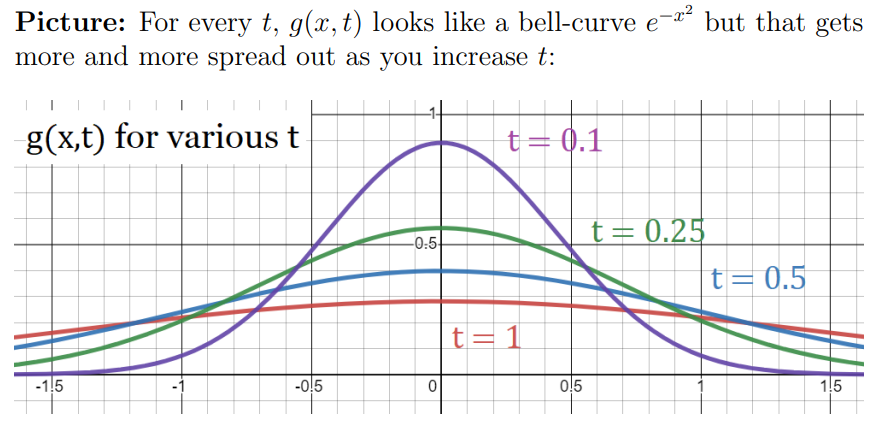
\includegraphics[width=0.8\textwidth]{Images/heat kernel.png}

Note that as $t \to 0^+$, $g(x, t)$ is the Dirac delta at $x = 0$

\subsection*{Part V - Convolution Intuition}
\textbf{Example:} What is the coefficient of $x^2$ in 
\[(x^2 + 2x + 3)(2x^2 + 4x + 1)\]

Generally, the coeff of $x^2$ in $(a_2x^2 + a_1x + a_0)(b_2x^2+ b_1x + b_2)$ is 
\[C_2 = a_0 b_2 + a_1 b_1 + a_2 b_0\] 
and more generally, the coefficient of $x^k$ in $(a_nx^n + ... a_0)(b_nx^n + ... + b_0)$ is 
\[C_k = \sum_{i=0}^k a_i b_{k-1}\]

Note the parallel to 
\[(f \star g)(x) = \int_{-\infty}^\infty f(y)\, g(x -y) \; dy\]

\section{Lecture 9: Feb 13}
\subsection*{Part I - Heat Equation Example}
\textbf{Example 1:} Solve 
\[\begin{cases}
    u_t = Du_{xx}\\
    u(x, 0) = e^{-x}
\end{cases}\]

\textbf{Solution:}
\[u(x, t) = \frac{1}{\sqrt4\pi D t} \int_{-\infty}^\infty e^{-\frac{(x - y)^2}{4Dt}} e^{-y} \; dy\]
Looking at the exponent:
\[\frac{-(x-y)^2}{4Dt} - y = -\frac{(x-y)^2 + 4Dty}{4Dt}\]
Expand the numerator:
\[ = -\frac{x^2 - 2xy - y^2 + 4Dty}{4Dt}\]
Note the numerator is a quadratic in y:
\begin{align*}
    y^2 + (4Dt - 2x)y + x^2 &= (y + 2Dt - x)^2 - (2Dt - x)^2 + x^2\\
    &= (y + 2Dt - x)^2 - 4D^2t^2 + 4Dtx - x^2 + x^2\\
    &= (y + 2Dt - x)^2 + 4Dt(x - Dt)
\end{align*}
So the full numerator is 
\[\frac{-(x-y)^2}{4Dt} = -\left(\frac{(y + 2Dt - x)^2 + 4Dt(x - Dt)}{4Dt}\right) = -\left(\frac{(y+2Dt-x)^2}{4Dt}+ (x - Dt)\right)\]
Substituting back in, 
\begin{align*}
    u(x, t) &= \frac{1}{\sqrt4\pi D t} \int_{-\infty}^\infty e^{-\left(\frac{(y+2Dt-x)^2}{4Dt}+ (x - Dt)\right)} \; dy\\
    &= \frac{e^{Dt - x}}{\sqrt4\pi D t}\int_{-\infty}^\infty e^{-frac{(y+2Dt-x)^2}{4Dt}} \; dy\\
    &= \frac{e^{Dt - x}}{\sqrt4\pi D t}\int_{-\infty}^\infty e^{-\left(\frac{y+2Dt-x}{\sqrt{4Dt}}\right)^2} \; dy\\
\end{align*}
Now use u-sub with 
\[p = \frac{y+2Dt-x}{\sqrt{4Dt}}\]
so 
\[dp = \frac{dy}{\sqrt{4Dt}} \implies dy = \sqrt{4Dt} \; dp\]
\[u(x, t) = \frac{e^{Dt - x}}{\sqrt{4\pi D t}}\int_{-\infty}^\infty e^{-p^2} \sqrt{4Dt}\; dp = \frac{e^{Dt - x}}{\sqrt{\pi}} \int_{-\infty}^\infty e^{-p^2}\; dp\]
\[\boxed{u(x, t) = e^{Dt- x}}\]

\subsection*{Part II - Infinite speed of propagation}
Remember the heat equation solution is:
\[u(x, t) = \frac{1}{\sqrt4\pi D t} \int_{-\infty}^\infty e^{-\frac{(x - y)^2}{4Dt}} f(y) \; dy\]
with an initial condition $u(x, 0) = f(x)$

\textbf{Property 1:} If $f \geq 0$ is positive somewhere and continuous, then $u(x, t)$ is positive everywhere. 

This means that heat propagates at infinite speed because heat at one place affects heat everywhere else instantly. Note that the transport equation implies a finite speed of propagation.

\textbf{Why?} 
Suppose $f(x_0) > 0$ for some $x_0$. Then because f is continuous it is actually positive for all x in an interval around $x_0$
Also 
\[u(x, t) = \frac{1}{\sqrt4\pi D t} \int_{-\infty}^\infty e^{-\frac{(x - y)^2}{4Dt}} f(y) \; dy\]
and we know the integrand is non-negative so we have 
\[\frac{1}{\sqrt4\pi D t} \int_{-\infty}^\infty e^{-\frac{(x - y)^2}{4Dt}} f(y) \; dy \geq \frac{1}{\sqrt4\pi D t} \int_{a}^b e^{-\frac{(x - y)^2}{4Dt}} f(y) \; dy\]
But the integrand of the second is also positive so 
\[u(x, t) > 0\] 

\subsection*{Part III  - Smoothness}
\textbf{Property 2:} $u(x, t)$ is infinitely differentiable (for $t >0$) even if $f(x)$ might not be 

\textbf{Why?}
All the derivatives fall of $\exp(-\frac{(x-y)^2}{4Dt})$ and not on f:
\[\frac{d}{dx} u(x, t) = \frac{d}{dx} \frac{1}{\sqrt4\pi D t} \int_{-\infty}^\infty e^{-\frac{(x - y)^2}{4Dt}} f(y) \; dy = \frac{1}{\sqrt4\pi D t} \int_{-\infty}^\infty \frac{d}{dx} e^{-\frac{(x - y)^2}{4Dt}} f(y) \; dy\]
But the term 
\[e^{-\frac{(x - y)^2}{4Dt}}\]
is infinitely differentiable and 
\[\frac{d}{dt}u(x, t) = Du_{xx}\]
but $u_{xx}$ is also smooth 

\subsection*{Part IV - Irreversibility}
\textbf{Property 3:} The heat equation is irreversible ($u(x, 0)$ cannot be determined from $u(x, 1)$)

\textbf{Why?}
"something something entropy"

Suppose $u(x, 1) = |x|$ but by smoothness, $u(x, t)$ must be smooth for all t so $|x|$ must be smooth but this is a contradiction

\section{Lecture 10: Feb 15}
\subsection*{Part I - Long-time behavior of the heat kernel}
\[u(x, t) = \frac{1}{\sqrt4\pi D t} \int_{-\infty}^\infty e^{-\frac{(x - y)^2}{4Dt}} f(y) \; dy\]

\textbf{Property 4:} 
\[\lim_{t \to \infty} u(x, t) = 0\]
"heat dissipates over time"

\textbf{Why?}
\begin{align*}
    |u(x, t)| &= \left|\frac{1}{\sqrt4\pi D t} \int_{-\infty}^\infty e^{-\frac{(x - y)^2}{4Dt}} f(y) \; dy\right|\\
    &\leq \frac{1}{\sqrt4\pi D t} \int_{-\infty}^\infty |f(y)| \underbrace{e^{-\frac{(x - y)^2}{4Dt}}}_{\leq 1} \; dy\\
    &\leq \frac{1}{\sqrt4\pi D t} \int_{-\infty}^\infty |f(y)| \; dy\\
    &= C \overset{t \to \infty}{\longrightarrow} 0
\end{align*}

\subsection*{Part II - Boundedness}
"u(x, t) does not blow up"

\textbf{Property 5: } If $|f(x) \leq M$ for some M (and all x) then for all x and t we have 
\[|u(x, t) \leq M\]

\textbf{Why?}
\begin{align*}
    |u(x, t)| &= \left|\frac{1}{\sqrt4\pi D t} \int_{-\infty}^\infty e^{-\frac{(x - y)^2}{4Dt}} f(y) \; dy\right|\\
    &\leq \frac{1}{\sqrt4\pi D t} \int_{-\infty}^\infty \underbrace{|f(y)|}_{\leq M} e^{-\frac{(x - y)^2}{4Dt}}\; dy\\
    &\leq \frac{M}{\sqrt4\pi Dt} \int_{-\infty}^\infty e^{-\left(\frac{y - x}{\sqrt{4\pi Dt}}\right)^2}\; dy \quad u = \frac{y - x}{\sqrt{4Dt}} \implies du = \frac{dy}{\sqrt{4Dt}}\\
    &= \frac{M}{\sqrt4\pi Dt} \int_{-\infty}^\infty e^{-u^2}\sqrt{4Dt}\; dy 
    &= \frac{M}{\sqrt4\pi Dt} \sqrt{4Dt} \sqrt{\pi}\\
    &= M
\end{align*}

\subsection*{Part III - Conservation of Mass}
"The area under the curve of u -- no matter its shape -- is always the same"

\[\int_{-\infty}^\infty u(x, t)\; dx =\int_{-\infty}^\infty f(x) \; dx \]

\textbf{Why?}

\emph{Lemma:} 
\[\lim_{x \to \pm \infty} u_x(x, t) = 0\]

Then,
\[u_t = Du_{xx}\]
\[\int_{-\infty}^\infty u_t(x, t)\; dx = \int_{-\infty}^\infty Du_{xx}(x, t)\; dx\]
and by FTC 
\[\frac{d}{dt}\int_{-\infty}^\infty u(x, t) \; dx = D\left[u_x(xm t)\right]_{-\infty}^\infty\]
Thus by the lemma,
\[\frac{d}{dt}\int_{-\infty}^\infty u(x, t) \; dx = D(0- 0) = 0\]
So the integral is constant with respect to time:
\[\int_{-\infty}^\infty u(x, t) \; dx = \int_{-\infty}^\infty u(x, 0) \; dx =\int_{-\infty}^\infty f(x) \; dx\]

\subsection*{Part IV - Inverse Fourier Transform}
Note that for the heat equation, we were very lucky to be able to write the Gaussian as a fourier transform
\[e^{-D\kappa^2t} = \F{\frac{1}{\sqrt{4\pi Dt}}e^{-\frac{x^2}{4Dt}}}\]
\textbf{But what do we do in general?}

Example: Solve 
\[\begin{cases}
    u_t = -u_{xxxx}\\
    u(x, 0) = f(x)
\end{cases}\]

Solution:
\begin{enumerate}
    \item Fourier transform it
    \[\F{u_t} = \F{-u_{xxxx}}\]
    \[\frac{d}{dt} \hat{u} = -(-i\kappa)^4 \hat{u} = -\kappa^4 \hat{u}\]
    \item Solve the ODE 
    \[\hat{u} = u(x, 0)e^{-\kappa^4t} = \hat{f}(\kappa) e^{-\kappa^4t} \]
    \item Write the exponential term as a fourier transform 
    
    \textbf{Definition:} \emph{Inverse Fourier Transform}
    \[\boxed{\check{f}(x) = \mathcal{F}^{-1}(x) = \frac{1}{2\pi} \int_{-\infty}^\infty f(\kappa) e^{-i\kappa x}\; d\kappa}\]

    So in this example, 
    \[e^{-\kappa^4t} = \hat{g}(\kappa) \quad g(x, t) = \mathcal{F}^{-1}\left(e^{-\kappa^4 t}\right) = \frac{1}{2\pi} \int_{-\infty}^\infty e^{-\kappa^4 t} e^{-i\kappa x}\; d\kappa\]

    \item Convolution 
    \item 
    So now we have 
    \begin{align*}
        \hat{u}(\kappa, t) &= \hat{f}(\kappa)e^{-\kappa^4 t}\\
        &= \hat{f}(\kappa) \hat{g}(\kappa, t)\\
        &= \F{f \star g}(\kappa, t)
    \end{align*}
    Therefore, 
    \[\boxed{\begin{cases}
        u(x, t) = \int_{-\infty}^\infty f(y) g(x - y)\; dy\\
        \text{where} \quad g(x, t) = \frac{1}{2\pi} \int_{-\infty}^\infty e^{-\kappa^4 t} e^{-i\kappa x}\; d\kappa
    \end{cases}}\]
\end{enumerate}

\section{Lecture 11: Feb 17}
\subsection*{Part I - The Wave Equation}
\[u_{tt} = c^2 u_{xx}\]
where $u = u(x, t)$ gives the displacement of a vibrating string at position x and time t and c is a constant giving the speed of the wave  

Note: despite the only difference between this and the heat equation is an extra time derivative, the derivation and solution will be \emph{completely} different

\subsection*{Part II - Derivation}
\begin{enumerate}
    \item Setting: start with a thin string of infinite length and consider a minute sub-piece from $x$ to $x + \Delta x$
    
    \textbf{Assumption:} points on the string only move vertically

    \item By Newton's second law of motion,
    \[F = ma\] 
    By the assumption above and the definition of u, the displacement vector is 
    \[s(x, t) = \brak{0, u(x, t)}\]
    Therefore, acceleration is 
    \[a(x, t) = s_{tt}(x, t) = \brak{0, u_{tt}}\]

    \textbf{Assumption:} the string has constant density $\rho$ 
    
    Then, the mass of the string is density times length (which can be taken by assuming the length is the hypotenuse of a right triangle with legs $\Delta x$ and $\Delta u$). Thus, 
    \[m = \rho \sqrt{(\Delta x)^2 + (\Delta u)^2}\]
    So,
    \[F = ma = \brak{0, \rho \sqrt{(\Delta x)^2 + (\Delta u)^2}}u_{tt}\]

    \item Study of the Force: 
    \textbf{Assumption: The only force acting on the string is the tension}
    So if $T(x, t)$ is the magnitude of the tension vector and $\theta(x, t)$ is the angle of the tension vector:

    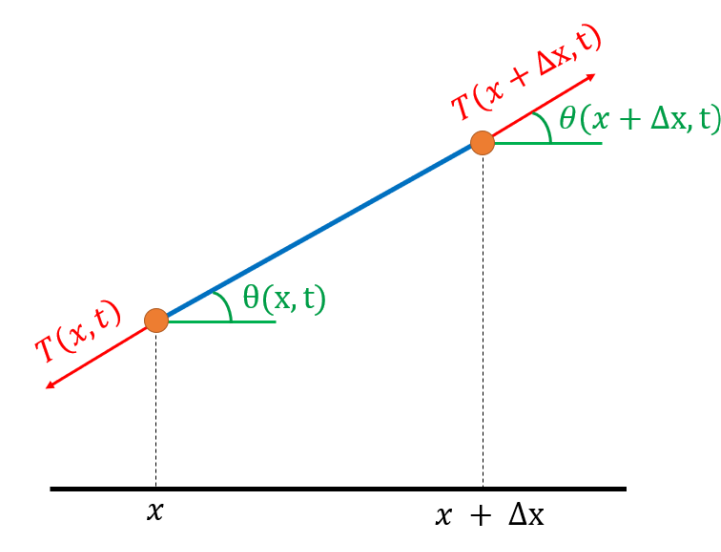
\includegraphics[width=0.8\textwidth]{Images/force.png}

    Then from trig, we can calculate the tension force via components of the resultant:
    \[\begin{cases}
        x = T(x, t) \cos(\theta(x, t))\\
        y = T(x, t) \sin(\theta(x, t))\\ 
    \end{cases} \Longrightarrow -\brak{T\cos(\theta), T\sin(\theta)}(x, t)\]
    Note: the minus comes from T pointing the opposite direction of the string

    Then in the same way, the force at $(x + \Delta x)$ is 
    \[\brak{T\cos(\theta), T\sin(\theta)}(x + \Delta x, t)\]

    so the net force is 
    \[F(x, t) = \brak{T\cos(\theta), T\sin(\theta)}(x + \Delta x, t) - \brak{T\cos(\theta), T\sin(\theta)}(x, t)\]

    \item Then using $F = ma$ and comparing the components, 
    \[\begin{cases}
        T\cos(\theta)(x + \Delta x, t) - T\cos(\theta)(x, t) = 0\\
        T\sin(\theta)(x + \Delta x, t) - T\sin(\theta)(x, t) = \rho \sqrt{(\Delta x)^2 + (\Delta u)^2} u_{tt}(x, t)
    \end{cases}\]
    Note, however, that both these LHS look like derivatives. 
    Starting with the cos terms,
    \[(T\cos(\theta))_x = 0\]
    so $T(x, t)\cos(\theta(x, t))$ is constant in x. 
    But $|\theta(x, t)| << 1$ so $\cos(\theta(x, t)) \approx 1$ and 
    \[T(x, t) \cos(\theta(x, t)) = T(x, t)\]
    which is constant in x so $T(x, t) = T(t)$ 

    \textbf{Assumption:} Tension is also constant in time $T(t) = T$

    Then the sin terms, 
    \begin{align*}
        (T\sin(\theta))_x &= \rho u_{tt} \left(\frac{\sqrt{(\Delta x)^2 + (\Delta u)^2}}{\Delta x}\right)\\
        &= \rho u_{tt} \sqrt{\frac{(\Delta x)^2 + (\Delta u)^2}{\Delta x}} \\
        &= \rho u_{tt}  \sqrt{1 + \left(\frac{\Delta u}{\Delta x}\right)^2} \\
        &= \rho u_{tt} \sqrt{1 + (u_x)^2}
    \end{align*}

    \textbf{Assumption:} if the displacements $\Delta u/\Delta x$ are small, then 
    \[\theta(x, t) = \tan^{-1}\frac{\Delta u}{\Delta x}\]
    is small, proving the inequality above. 

    Then, as $\Delta x \to 0$, $|u_x| << 1$ so 
    \[\sqrt{1 + (u_x)^2} \approx 1\]
    and 
    \[(T\sin(\theta))_x = \rho u_{tt}\]
    but 
    \[\sin \theta  = \tan \theta \cos \theta = \frac{\Delta u}{\Delta x} \cos \theta \to u_x\]
    so 
    \[(Tu_x)_x = Tu_{xx} \quad (\text{assuming T is constant})\] 
    and at last, 
    \[Tu_{xx} = \rho u_{tt} \longrightarrow u_{tt} = \frac{T}{\rho}u_{xx}\]
    Set, $c = \sqrt{T / \rho} > 0$ and 
    \[\boxed{u_{tt} = c^2 u_{xx}}\]
\end{enumerate} 

\section{Lecture 12: Feb 22}
\textbf{Goal:} Solve $u_{tt} = c^2 u_{xx}$
\subsection*{Part I - Factoring Method}
But this kind of looks like 
\[t^2 - c^2 x^2 = (t - cx)(t + cx)\]

\textbf{Definition:} Differential operator
\[\frac{\partial}{\partial t} u = u_t\]
\[\left(\frac{\partial}{\partial t}\right)^2 u = u_{tt}\]

Using this operator we can more rigorously "factor" the PDE.

\begin{enumerate}
    \item Apply the differential operator 
    \begin{align*}
        u_{tt} - c^2 u_{xx} &= \left[\left(\frac{\partial}{\partial t}\right)^2 - c^2 \left(\frac{\partial}{\partial x}\right)^2\right]u\\
        &= \left(\frac{\partial}{\partial t} - c \frac{\partial}{\partial x}\right)\left(\frac{\partial}{\partial t} + c \frac{\partial}{\partial x}\right)
    \end{align*}
    \item Solve the equation 
    \[u_{tt} - c^2 u_{xx} = 0\]
    \[\left(\frac{\partial}{\partial t} - c \frac{\partial}{\partial x}\right)\left(\frac{\partial}{\partial t} + c \frac{\partial}{\partial x}\right) = 0\]
    Let $v = \left(\frac{\partial}{\partial t} + c \frac{\partial}{\partial x}\right)u$ 
    so 
    \[\left(\frac{\partial}{\partial t} - c \frac{\partial}{\partial x}\right)v = 0 \Longrightarrow v_t - cV_x = 0\]
    \item Solve the transport PDE 
    \[v(x, t) = f(x + ct)\]
    \item Solve for u 
    \[v := \left(\frac{\partial}{\partial t} + c \frac{\partial}{\partial x}\right)u = u_t + cu_x\]
    \[u_t + cu_x = f(x + ct)\]
    But this is just an inhomogeneous transport equation! 
    The homogeneous solution is just 
    \[u_0(x, t)= G(x - ct)\]
    And a particular solution can be found using undetermined coefficients. Notice that the RHS is a function of $x +ct$ so we can guess 
    \[u_p = h(x + ct)\]
    so 
    \[(h(x + ct))_t + c(h(x + ct))_x = f(x + ct)\]
    \[ch'(x+ ct) + ch'(x + ct) = f(x + ct)\]
    \[2ch'(x + ct) = f(x + ct) \Longrightarrow h' = \frac{1}{2c}f'\]
    \[h(x + ct) = \frac{1}{2c}F(x + ct)\]
    where $F$ is an antiderivative of $f$
    Thus giving the general solution
    \[u(x, t)= G(x - ct) + \frac{1}{2c}F(x + ct) \]
    \[\boxed{u(x, t) = G(x - ct) + F(x + ct)}\]
\end{enumerate}

\textbf{Interpretation:} A wave is a sum of two functions, one moving to the left at speed c and the other to the right at speed c 

\subsection*{Part II - Coordinate Method}
\begin{enumerate}
    \item Define variables 
    \[\begin{cases}
        \xi  =x - ct \\
        \eta = x + ct
    \end{cases}\]
    \item Chain rule 
    \[u_x = \frac{\partial u}{\partial \xi} \frac{\partial \xi}{\partial x} + \frac{\partial u}{\partial \eta} \frac{\partial \eta}{\partial x} = u_\xi + u_\eta\]
    and 
    \begin{align*}
        u_{xx} = (u_x)_x &= \frac{\partial u_x}{\partial \xi} \frac{\partial \xi}{\partial x} + \frac{\partial u_x}{\partial \eta} \frac{\partial \eta}{\partial x} \\
        &= u_{\xi_\xi} + u_{\eta_\eta} = u_{\xi \xi} + u_{\eta \xi} + u_{\xi \eta} + u_{\eta \eta}\\
        &= u_{\xi \xi} + 2u_{\xi \eta} + u_{\eta \eta}
    \end{align*}
    Similarly, 
    \[u_tt = c^2 (u_{\xi \xi} - 2u_{\xi \eta} + u_{\eta \eta})\]

    \item Plug into wave equation:
    \[u_tt = c^2 u_{xx}\]
    \[c^2 (u_{\xi \xi} - 2u_{\xi \eta} + u_{\eta \eta}) = c^2( u_{\xi \xi} + 2u_{\xi \eta} + u_{\eta \eta}) = 4u_{\xi \eta}\]
    \[\boxed{u_{\xi \eta} = 0}\]
\end{enumerate}

\section{Lecture 13: Feb 24}
\subsection*{Part I - Solving the wave equation (continued)}
\[u_{tt} = c^2 u_{xx}\]
Using the coordinate method with the choices 
\[\begin{cases}
    \xi = x - ct\\
    \eta = x + ct
\end{cases}\]
we get the equation 
\[u_{\xi \eta} = 0\]
so
\[u_\xi = f(\xi) \Longrightarrow u = F(\xi) + G(\eta)\]
thus 
\[\boxed{u(x, t) = F(x - ct) + G(x + ct)}\]

\subsection*{Part II - D'Alembert's Formula}
\textbf{Example:}
\[\begin{cases}
    u_{tt} = c^2 u_{xx}\\
    u(x, 0) = \phi(x)\\
    u_t(x, 0) = \psi(x)
\end{cases}\]

\textbf{Solution:}
\begin{enumerate}
    \item General Solution
    \[u(x, t) = F(x - ct) + G(x + ct)\]
    \item Plug in the initial condition
    \[u(x, 0) = \phi(x) = F(x) + G(x)\]
    \item Differentiate with t 
    \[u_t(x, t) = -cF'(x - ct) + cG(x + ct)\]
    \[u_t(x, 0) = \psi(x) = -cF'(x) + cG'(x)\]
    \[-F'(x) + G'(x) = \frac{\psi(x)}{c}\]
    \item Integrate over $[0, x]$
    \[\int_0^x -F'(s) + G'(s) \; ds = \int_0^x \frac{\psi(s)}{c} \; ds\]
    \[-F(x) + G(x) - (-F(0) + G(0)) = \frac{1}{c} \int_0^x \psi(s) \; ds\]
    This gives us the system of equations
    \[\begin{cases}
        -F(x) + G(x) = A + \frac{1}{c} \int_0^x \psi(s) \; ds\\
        F(x) + G(x) = \phi(x)
    \end{cases}\]
    \[\Longrightarrow \begin{cases}
        2G(x) = \phi(x) + A + \frac{1}{c} \int_0^x \psi(s) \; ds\\
        2F(x) = \phi(x) - A - \frac{1}{c} \int_0^x \psi(s) \; ds\\
    \end{cases} \Longrightarrow \begin{cases}
        F(X) = \frac{1}{2}\phi(x) - \frac{A}{2} - \frac{1}{2c}\int_0^x \psi(s) \; ds\\
        G(X) = \frac{1}{2}\phi(x) + \frac{A}{2} + \frac{1}{2c}\int_0^x \psi(s) \; ds\\
    \end{cases}\]
    \item Solution 
    \begin{align*}
        u(x, t) &= F(x - ct) + G(x + ct)\\
        &= (\frac{1}{2}\phi(x - ct) - \frac{A}{2} - \frac{1}{2c}\int_0^{x- ct}\psi(s) \; ds) \\
        &\quad + (\frac{1}{2}\phi(x + ct) \frac{A}{2} + \frac{1}{2c}\int_0^{x + ct} \psi(s) \; ds)\\
        &= \frac{1}{2}(\phi(x - ct) + \phi(x + ct)) + \frac{1}{2c}\left(\int_{x-ct}^0 \psi(s)\; ds + \int_0^{x  +ct} \psi(s) \; ds\right)\\
    \end{align*}

    Which at last gives us d'Alembert's equation to solve the wave equation with initial conditions:
    \[\boxed{u(x, t) = \frac{1}{2}(\phi(x - ct) + \phi(x + ct)) + \frac{1}{2c}\int_{x - ct}^{x + ct} \psi(s)\;ds}\]
\end{enumerate}

\subsection*{Part III  - Example}
\[\begin{cases}
    u_{tt} = u_{xx}\\
    u(x, 0) = 0\\
    u_t(x, 0) = \cos(x)\\
\end{cases} \implies \begin{cases}
    c = 1\\
    \phi(x) = 0\\
    \psi(x) = \cos (x)
\end{cases}\]
Then using D'Alembert's:
\begin{align*}
    u(x, t) &= \frac{1}{2}(\phi(x - ct) + \phi(x + ct)) + \frac{1}{2c}\int_{x - ct}^{x + ct} \psi(s)\;ds\\
    &= \frac{1}{2}(0 + 0) + \frac{1}{2} \int_{x - t}^{x +t}\cos(s)\; ds\\
    &= \frac{1}{2}(\sin(x + t) - \sin(x - t))\\
    &= \frac{1}{2}(\sin x \cos t + \cos x \sin t - \sin x \cos -t - \cos x \sin -t)\\
    &= \frac{1}{2}(2 \cos x \sin t)
\end{align*}
\[\boxed{u(x, t) = \sin(t) \cos(x)}\]
(Or, the wave takes the shape of cos with amplitude sin)

\
\end{document}  
